\documentclass[border=10pt]{standalone}
\usepackage{pgfplots}
\pgfplotsset{compat=1.18}
\begin{document}
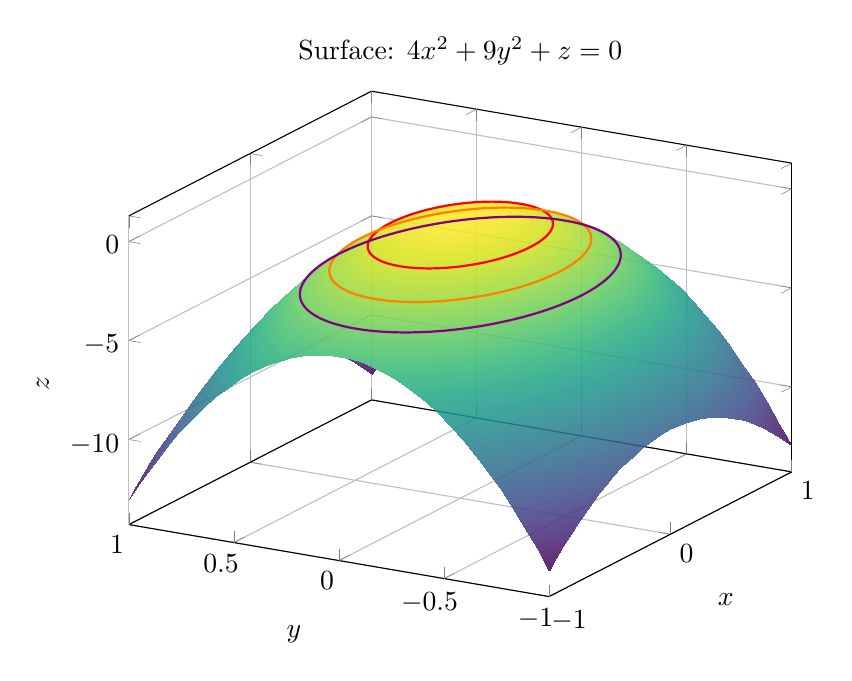
\begin{tikzpicture}
\begin{axis}[
  width=10cm, height=8cm,
  xlabel=$x$, ylabel=$y$, zlabel=$z$,
  title={Surface: $4x^2+9y^2+z=0$},
  view={-60}{25},
  domain=-1:1,
  y domain=-1:1,
  samples=35,
  samples y=35,
  colormap/viridis,
  grid=major
]
\addplot3[surf, shader=interp, opacity=0.85] {-4*x^2-9*y^2};
\addplot3+[domain=0:2*pi, samples=120, no marks, thick, red]
  ({sqrt(1/4)*cos(deg(x))},{sqrt(1/9)*sin(deg(x))},{-1});
\addplot3+[domain=0:2*pi, samples=120, no marks, thick, orange]
  ({sqrt(2/4)*cos(deg(x))},{sqrt(2/9)*sin(deg(x))},{-2});
\addplot3+[domain=0:2*pi, samples=120, no marks, thick, violet]
  ({sqrt(3/4)*cos(deg(x))},{sqrt(3/9)*sin(deg(x))},{-3});
\end{axis}
\end{tikzpicture}
\end{document}